\newpage
\section{Original Tech Review}
\def\TRtitle{Computer Science Senior Software Engineering Project (CS462)}
\def\TRterm{Winter 2017}

	\begin{center}
		\vspace{\fill}

		{\Huge\bfseries Original Tech Review\par}
		\vspace{0.5cm}
		{\Large\itshape \TRtitle\par}
		\vspace{0.5cm}
		{\Large\itshape \TRterm\par}
		
		\vspace{\fill}
	\end{center}
	
	\begin{abstract}
		This project is a proof concept to explore a potential technological innovation for Head-Up Display (HUD) system that present critical flight information to pilots. The primary objective of this project is to reduce the cost and time required to precisely align flight information to the HUD by introducing additional sensor to the system to make the alignment process more dynamic. To achieve this goal, there are eight different main technologies that will be critical for the development of the project. This document will compare three alternative options for each main technologies. This document will also include the option that we choose for each main technologies to develop this project. 
	\end{abstract}
	
	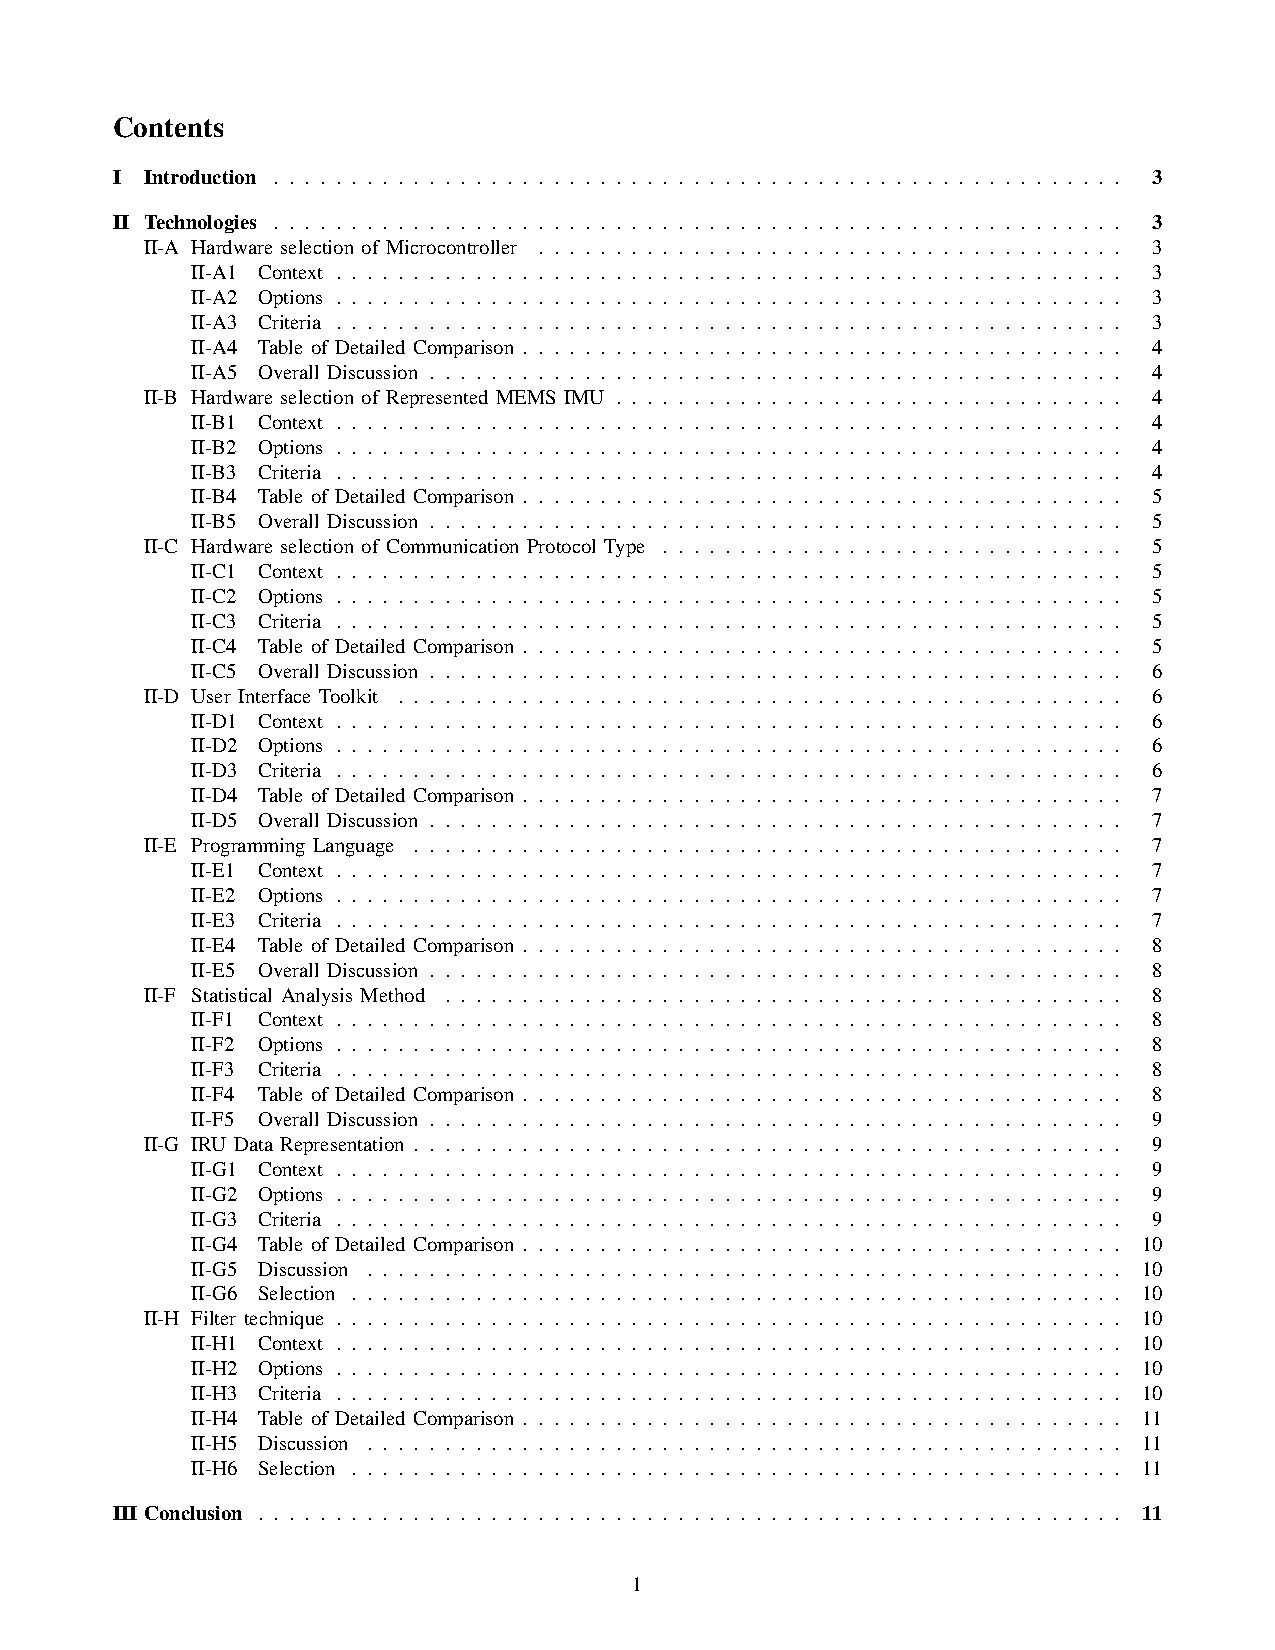
\includepdf[pages=-]{pdf/tech_review.pdf}

	\subsection{Necessary Change Based on Original Technology}
		\subsubsection{Change in D.User Interface Toolkit}
			Our previous GUI have a 2D gauge-like looks to it. It looks more like a car dashboard rather than a real plane HUD. This GUI serve our purpose of showing the data well. However, it is hard to visualize the change on the plane for each angle. Our team is determined to give the best for this project and decided to improve on our GUI. To solve this problem, we create a new GUI that visualize the change of angle to a plane object. We create this GUI by using a python library called VPython. We also use the pySerial library to connect the GUI to the Arduino part of the project, an new overall review seen as following:\\

			\begin{itemize}
				\item \textbf{Complexity:}
				least complex

				\item \textbf{Accessibility:}
				Free open source

				\item \textbf{Adoption Rate:}
				Few tutorials or examples

				\item \textbf{Time Commitment:}
				Minimal

				\item \textbf{Library:}
				Powerful
				
				\item \textbf{Overall Cost and Benefit:}
				Easy but powerful, but too few online tutorials could be found\\
			\end{itemize}

		\subsubsection{Change in F.Statistical Analysis Method}
			For our statistical analysis, we ended up applying a 95\% confidence interval to our offset data to ensure that the resulting offset was precise. Confidence interval is easier to be programmed but it also works well. In addition, by using a confidence interval, we can retrieve a valid offset value as soon as the quaternion value converges. Without using a confidence interval, we could end up with an erroneous value.











